

\section{Methods and Results}

In this section we explore ...

\subsection{Costing Energy Retrofits and their impacts}
Dwellings with at least one inspection recording an EPC ($15.6$ million registered), were analysed. Each EPC records current and potential energy efficiency, rating, retrofits available together with recommendation file which lists potential retrofits in a given property.

Should the property be able to raise their EPC, the record will include the potential energy rating alongside their current energy rating, respectively denoted $R_p$ and $R_c$ in the equation below, so that the difference in energy efficiency is explained by committing to specific retrofits (with $R_i$ a list of retrofits):
\begin{align*}
    E_{i,p} - E_{i,c} = f(R_{i})
\end{align*}
%In cases where the minimum or maximum costs were missing, only the given value was taken into account. For each improvement ever recommended on an EPC, each of its attributes advertised were stored, dated and averaged with its other appearances for dwelling having undergone an inspection the same year. Differences were taken across all attributes. If an improvement was no longer recommended, it was assumed it must have been implemented between inspections. This identification strategy enabled to explore a wider sample dataset than previously attempted by surveys (Coyne and Denny, 2021).\\
\noindent We start with estimating the impact of distinct energy retrofits on a series of dependent variables, including Energy Efficiency, energy consumption, costs and emissions in a given dwelling. We run the following regression using Ordinary Least Square (OLS):
\begin{align}
    Y_i = E_{i,p} -E_{i,c} = \beta_0 + \sum_{m=1}^{63} \beta_{\text{m}} X_{\text{i,m}}  + \gamma_i \cdot time_{fe} +  \epsilon_i
\label{eq:general_impacts_OLS}
\end{align}
where $Y_i$ captures Energy Efficiency (score out of 100), Yearly energy Consumption ($kWh/m^2$), costs (\textsterling  \textbackslash $kWh$) and $CO_2$ emissions. $X_{i,m}$ is a vector of energy retrofits in a given property $i$. The environmental impact ratings are based on the carbon emissions of buildings per square meter \cite{rowe_housing_2024}. Time fixed effects are captured by $time_{fe}$ and $\epsilon_i$ is the error term. \\

Results from the five OLS regressions (Eq. \ref{eq:general_impacts_OLS}) are presented in Table \ref{tab:ID_impacts} below. Coefficients are all significant (p-value less than 0.0001).  They provide insight into the marginal effects of each completed structural retrofit on the energy efficiency score, energy consumption (in kWh and £), and emissions (in CO2 and impact score) of dwellings. According to table \ref{tab:ID_impacts}, installing a wood pellet stove with boiler and radiator (ID 23 \& 39) can increase a property’s energy efficiency rating by 22.79, making this improvement option the most optimal decision when aiming to increase the EPC score ($Y_1$). As expected, improvement ID 23\&39, also yields the greatest impact with all other dependent variables, resulting in the most impact retrofit available to homeowners from a purely results-based perspective. When comparing across all the regression results, it seems the most ’impactful’ renovations involve improving a dwelling’s heating systems (e.g., Fan assisted storage heaters,
gas condensing boilers, replacing heating units, etc.). This is consistent with prior findings that the majority of residential energy consumption and associated emissions stem from space and water heating \cite{lowe_technical_2007, kesicki_costs_2012} . Conversely, the recommendations associated with the lowest impact estimates from the models, are mostly associated with fabric energy efficiency and energy conservation measures (i.e., loft insulation, double window glazing, party wall insulation, etc.). The results were appended and used during the subsequent parts of the analysis as indicators of impacts for each dwelling.  
\begin{table}[h!] 
\begin{center}
\caption{Regressions Results: Impacts of Improvements according to EPCs 2008-22}
\label{tab:ID_impacts}
\resizebox{\textwidth}{!}{ 
\begin{tabular}{r p{5cm} rrrrr | r} 
\toprule
\toprule
&   &  \multicolumn{5}{c}{\textit{Dependent Variables}}  \\
\cmidrule(lr){3-7}  % Partial midrule 
&   & \textbf{EPC(\%)} & \textbf{Consumption (kWh)} & \textbf{CO2} & \textbf{Environmental} & \textbf{Bill (\textsterling)} \\ 
 & \textit{Independent Variables} &   ($Y_1$) & ($Y_2$) & ($Y_3$) & ($Y_4$) & ($Y_5$) & \textbf{Cost (\textsterling)}\\ 
\midrule
\midrule
1-3 & Insulate hot water cylinder with 80 mm jacket & $3.66^{***}$ & $-40.56^{***}$ & $-0.37^{***}$ & $3.93^{***}$ & $-62.25^{***}$ & $22.5$ \\ 
4 & Hot water cylinder thermostat  & $4.48^{***}$ & $-32.83^{***}$ & $-0.66^{***}$ & $4.78^{***}$ & $-121.14^{***}$ & $300$\\ 
5 & Increase loft insulation to 270 mm  & $3.20^{***}$ & $-26.05^{***}$ & $-0.45^{***}$ & $3.74^{***}$ & $-93.96^{***}$ & $225$\\ 
6 & Cavity wall insulation  & $4.79^{***}$ & $-40.68^{***}$ & $-0.64^{***}$ & $5.48^{***}$ & $-126.39^{***}$ & $1000$\\ 
7 & 50 mm internal or external wall insulation & $6.30^{***}$ & $-52.08^{***}$ & $-0.89^{***}$ & $7.01^{***}$ & $-186.02^{***}$ & $9000$\\ 
8 & Replace single glazed windows with low-E double glazing  & $2.31^{***}$ & $-21.55^{***}$ & $-0.45^{***}$ & $2.22^{***}$ & $-90.07^{***}$ & $4900$\\ 
9 & Secondary glazing to single glazed windows & $2.44^{***}$ & $-12.72^{***}$ & $-0.66^{***}$ & $1.26^{***}$ & $-110.11^{***}$ & $1250$\\ 
10 & Draughtproof single-glazed windows  & $4.46^{***}$ & $-28.88^{***}$ & $-1.01^{***}$ & $3.99^{***}$ & $-198.74^{***}$ & $100$\\ 
11-18 & Upgrade heating controls  & $2.29^{***}$ & $-15.11^{***}$ & $-0.32^{***}$ & $2.60^{***}$ & $-62.79^{***}$ & $400$ \\ 
19 & Solar water heating  & $2.84^{***}$ & $-30.54^{***}$ & $0.47^{***}$ & $3.20^{***}$ & $84.64^{***}$ & $5000$\\ 
20-21 & Replace boiler with new condensing boiler  & $4.39^{***}$ & $-33.06^{***}$ & $-0.75^{***}$ & $5.53^{***}$ & $-139.94^{***}$ & $2550$\\ 
22 & Replace boiler with biomass boiler  & $14.62^{***}$ & $-106.26^{***}$ & $-11.78^{***}$ & $57.12^{***}$ & $-585.71^{***}$ & $10000$\\ 
23\&39 & Wood pellet stove with boiler and radiators  & $22.79^{***}$ & $-234.00^{***}$ & $-14.62^{***}$ & $58.98^{***}$ & $-1161.85^{***}$ & $10000$\\ 
24\&30 & Fan assisted storage heaters and Dual Immersion Cylinder & $9.19^{***}$ & $-58.68^{***}$ & $-0.75^{***}$ & $4.89^{***}$ & $-179.76^{***}$ & $1123.8$\\ 
25\&31 & Fan-assisted storage heaters & $9.19^{***}$ & $-58.68^{***}$ & $-0.75^{***}$ & $4.89^{***}$ & $-179.76^{***}$ & $998.75$\\ 
26 & Replacement warm air unit & $2.38^{***}$ & $-14.73^{***}$ & $-0.38^{***}$ & $3.00^{***}$ & $-95.81^{***}$ & $1875$\\ 
27,29,32,40-42 & Change heating to gas condensing boiler & $18.36^{***}$ & $-173.60^{***}$ & $-2.20^{***}$ & $17.87^{***}$ & $-586.96^{***}$ & $5000$\\ 
28\&43 & Condensing oil boiler with radiators & $10.24^{***}$ & $-18.21^{***}$ & $-2.72^{***}$ & $7.53^{***}$ & $-429.72^{***}$ & $12500$\\ 
34 & Solar photovoltaic panels, 2.5 kWp  & $6.41^{***}$ & $-27.92^{***}$ & $-1.47^{***}$ & $5.01^{***}$ & $-145.52^{***}$ & $4500$\\ 
35 & Low energy lighting for all fixed outlets  & $0.88^{***}$ & $-5.38^{***}$ & $-0.11^{***}$ & $0.82^{***}$ & $-35.12^{***}$ & $30.40$\\ 
36 & Replace heating unit with condensing unit  & $2.92^{***}$ & $-22.77^{***}$ & $-0.40^{***}$ & $3.50^{***}$ & $-83.92^{***}$ & $2600$ \\ 
37-38 & Install condensing boiler  & $13.65^{***}$ & $-47.16^{***}$ & $-3.99^{***}$ & $11.48^{***}$ & $-680.93^{***}$ & $2600$\\ 
44 & Wind turbine & $6.20^{***}$ & $-37.59^{***}$ & $-0.87^{***}$ & $4.66^{***}$ & $-70.00^{***}$ & $19999.3$\\ 
45 & Flat roof insulation  & $4.05^{***}$ & $-35.29^{***}$ & $-0.60^{***}$ & $4.49^{***}$ & $-132.82^{***}$ & $1175$\\ 
46 & Room-in-roof insulation & $7.57^{***}$ & $-49.07^{***}$ & $-1.92^{***}$ & $8.32^{***}$ & $-398.64^{***}$ & $2100$\\ 
47 & Floor insulation & $5.41^{***}$ & $-33.05^{***}$ & $-0.63^{***}$ & $6.38^{***}$ & $-88.26^{***}$ & $1000$\\ 
48 & High performance external doors & $5.07^{***}$ & $-50.21^{***}$ & $-0.22^{***}$ & $3.50^{***}$ & $-77.32^{***}$ & $1365.6$ \\ 
49 & Heat recovery system for mixer showers & $1.49^{***}$ & $-50.21^{***}$ & $-0.09^{***}$ & $1.01^{***}$ & $-50.43^{***}$ & $655$\\ 
50 & Flue gas heat recovery device in conjunction with boiler & $3.81^{***}$ & $-42.05^{***}$ & $0.56^{***}$ & $2.85^{***}$ & $80.30^{***}$ & $650$\\ 
56 & Replacement glazing units  & $1.49^{***}$ & $-16.67^{***}$ & $-0.15^{***}$ & $2.24^{***}$ & $-29.63^{***}$ & $1200$\\ 
57 & Suspended floor insulation  & $4.01^{***}$ & $-32.61^{***}$ & $-0.58^{***}$ & $4.65^{***}$ & $-114.17^{***}$ & $1000$\\ 
58 & Solid floor insulation & $4.44^{***}$ & $-34.68^{***}$ & $-0.64^{***}$ & $4.62^{***}$ & $-112.41^{***}$ & $5000$\\ 
59\&61 & High heat retention storage heaters and dual immersion cylinder & $17.32^{***}$ & $-85.81^{***}$ & $-0.72^{***}$ & $4.21^{***}$ & $-489.40^{***}$ & $1501.3$\\ 
60\&62 & High heat retention storage heaters & $9.14^{***}$ & $-64.51^{***}$ & $-0.49^{***}$ & $3.55^{***}$ & $-249.02^{***}$ & $1346.1$\\ 
63 & Party wall insulation & $2.53^{***}$ & $-32.71^{***}$ & $-0.14^{***}$ & $3.30^{***}$ & $-24.36^{***}$ & $450$\\
\addlinespace
\midrule
& Year Fixed.E     & \textit{yes}    & \textit{yes}  & \textit{yes} & \textit{yes} & \textit{yes} \\
& Efficiency Gradings    & \textit{yes}    & \textit{yes}  & \textit{yes} & \textit{yes} & \textit{yes} \\
\bottomrule
\bottomrule
\end{tabular}
}
\end{center}
\caption*{\scriptsize{\textit{\small{\textbf{NOTES:} These estimates are the results of OLS regressions. The table reports the impacts of each improvement (independent variables). The coefficients represent the change in the dependent variables per improvement completed (independent variable). The columns report the estimated impact of each improvement on the change in EPC($Y_1$), change in Energy Consumption($Y_2$), $CO_2$ emissions ($Y_3$), Environmental Impact factor ($Y_4$), and total energy costs in ($Y_5$). Regressions include household fixed effects, along with time controls in the second column. Robust standard errors in parentheses. Significance levels are indicated as $^{***}p<0.001$; $^{**}p<0.01$; $^{*}p<0.05$}}}}

\end{table}


\subsection{Cumulative costs and environmental impacts of reaching EPC-C}

As previously mentioned, property owners are not obligated but highly encouraged to follow the ordered improvement suggestions on the EPC \cite{department_for_communities_and_local_government_guide_2017}. Figure \ref{fig:decision_models} provides an overview of the 3 'retrofitting strategies' used to model the complex decision-making process of property owners willing to retrofit. Faced with the EPC recommendations lists, owners can opt for the 'low hanging fruit' improvements if faced with requirements to retrofit and low financial capabilities \cite{jones_retrofitting_2013}. In this strategy, it is assumed the cheapest structural retrofitting suggestions would be firstly implemented. Conversely, the strategy 4 would highlight dwellings willing to invest first in improvements that could yield the highest impact (change in EPC score) to retrofit with minimal interventions. Finally, a more complex scenario is explored (strategy 3). In this model, it is assumed homeowners could estimate the 'highest impact per pound' improvements and preferably selected such impactful and worth-while retrofits. \\

\begin{figure}[h!]
    \centering
    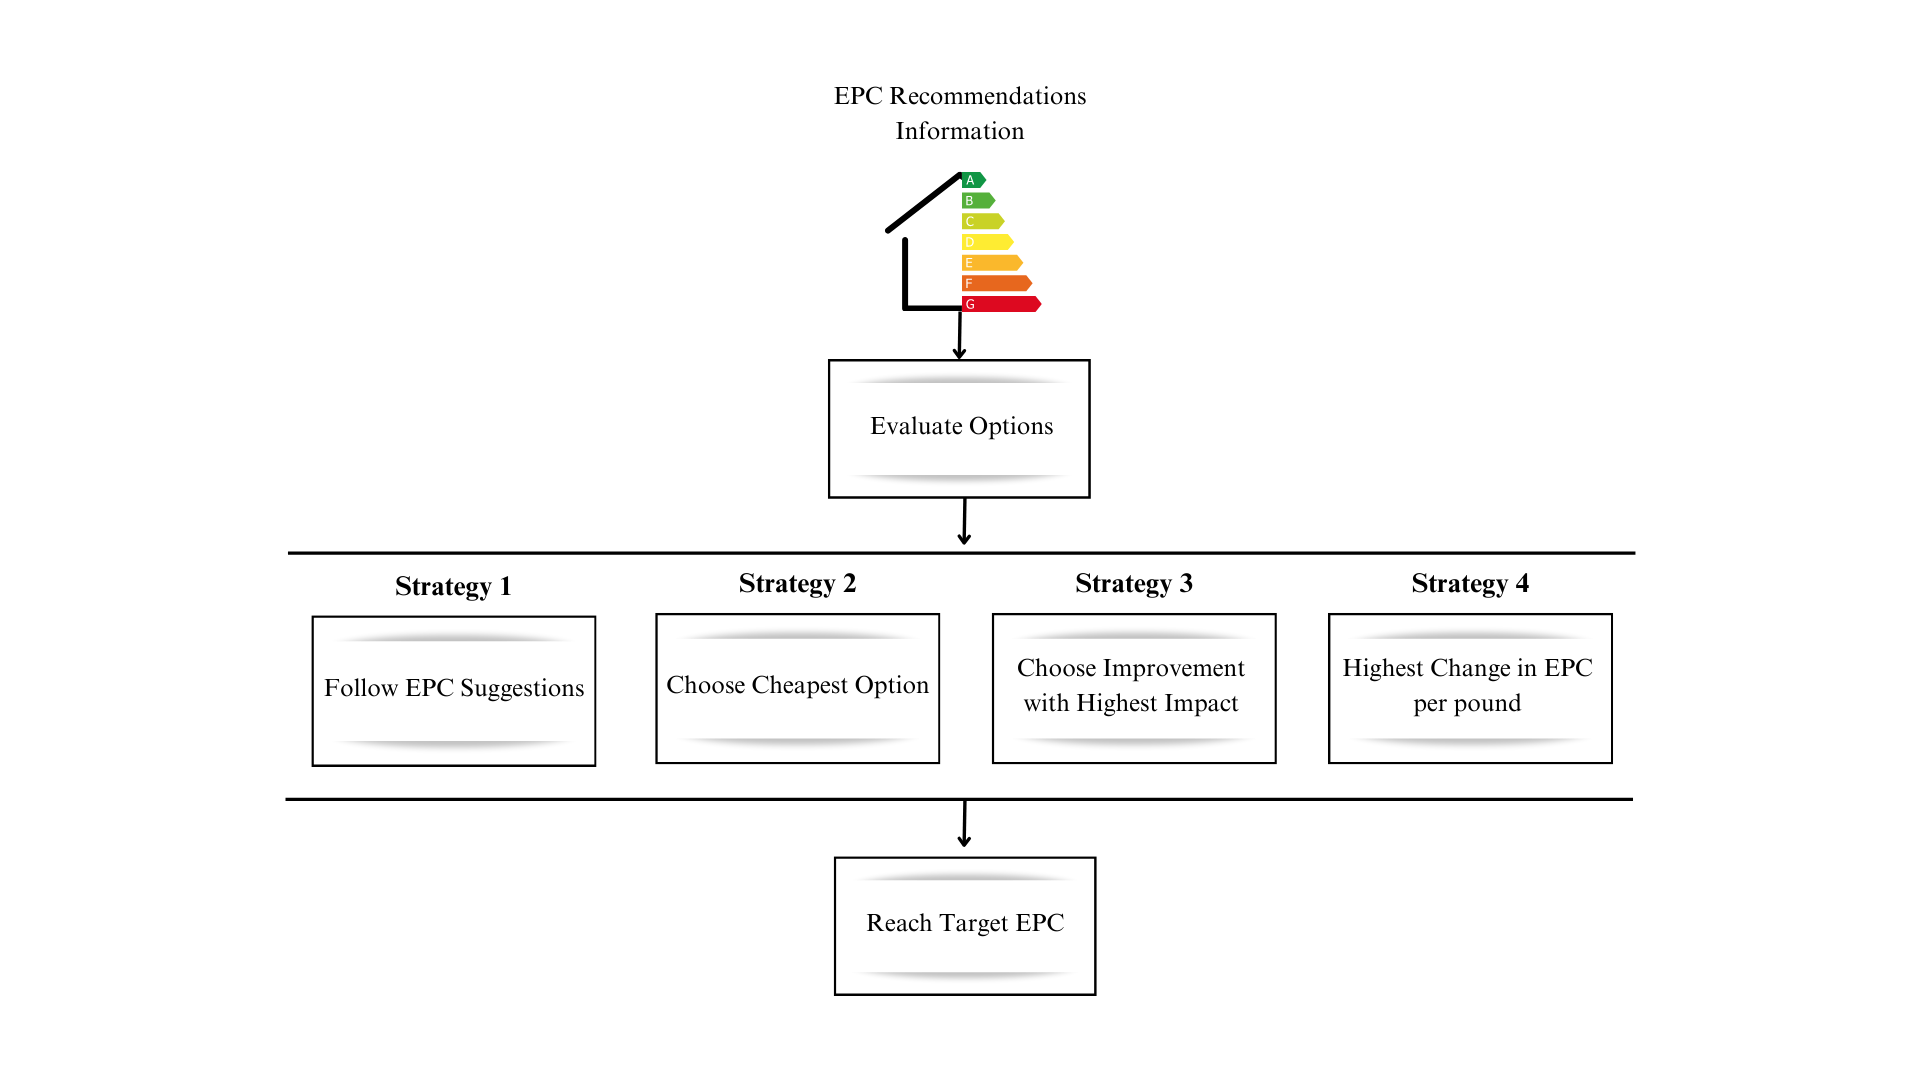
\includegraphics[width=1\linewidth]{src/figures/decision_model.png}
    \caption{Conceptual framework of decision models used to estimate cost of reaching minimum energy efficiency. The strategies were executed as separate rule-based algorithms applied to the latest energy performance certificates for every unique properties.}
    \label{fig:decision_models}
\end{figure}


The cumulative costs of achieving the EPC cap was determined for each nuanced retrofitting strategy: 1) per EPC recommendation, 2) as per EPC impact potential, 3) cheapest improvement option) and 4) by best impact per investment (EPC\_impact/Cost of retrofit). The program ran on the $9.2$ million dwellings that were able to rise their EPCs and had an original energy efficiency below that of the MEES amendment suggested of $69\%$ (C-Band).  The linear estimation models overestimated the cumulative and individual costs and impacts of reaching the minimum EPC rating standards (Table \ref{EPC_69_costs}). This was probably induced as the linear estimation included some costly improvements at the of the EPC recommendations which would have yielded more than the necessary scores. Conversely, the computationally-determined costs using different 'strategies' stopped keeping track of structural improvements once households reached the set threshold. The total costs for retrofitting all able registered properties in England and Wales to an EPC rating of C range from \textsterling 59 billion to \textsterling 94 billion, allowing the sector to reduce its yearly emissions by 18.1 - 20 million tonnes of $CO_2{eq}$. In 2023, residential emissions from buildings in the UK accounted for 51.7 million tones of $CO_2{eq}$ \footnote{2023 Provisional figures from ONS and DESNZ}. The cumulative costs would be estimated at about \textsterling 82.5 billion if all home owners followed and implemented the list of recommendations provided by their EPCs. For each investment strategy, the cumulative change in energy consumption for the housing sector is also displayed and presented in $GWh/m^2$. While the EPC retrofitting strategy does not yield the greatest decrease in emissions, SAP recommendations allow for the most significant decrease in energy consumption. \\

% Include the table on total costs
% add ordered by carbon reduction, remove ENv column
\begin{table}[!h]
\caption{Cumulative Costs for EPC Cap 69}
\label{EPC_69_costs}
\centering
\resizebox{\ifdim\width>\linewidth\linewidth\else\width\fi}{!}{
\begin{tabular}[t]{lrlrrrr}
\toprule
\toprule
 & \textbf{N. Retrofits} & \textbf{Household} (\textsterling) & \textbf{CO2 ($MtCO_eq/yr$)} & \textbf{Env}($MtCO_eq/yr$)  & \textbf{Energy ($GWh/m^2$)} & \textbf{Total Cost} (\textsterling)\\

\midrule

\cellcolor{gray!10}{By Yield}  & \cellcolor{gray!10}{3} & \cellcolor{gray!10}{6597} & \cellcolor{gray!10}{-18.6} & \cellcolor{gray!10}{124.4} & \cellcolor{gray!10}{-881.6} & \cellcolor{gray!10}{60,887,982,229}\\

By Price & 3 & 6670 & -18.3 & 124.6 & -885.2 & 61,558,192,060\\

\cellcolor{gray!10}{By EPC} & \cellcolor{gray!10}{3} & \cellcolor{gray!10}{9058} & \cellcolor{gray!10}{-16.1} & \cellcolor{gray!10}{125.3} & \cellcolor{gray!10}{-918.3} & \cellcolor{gray!10}{83,179,781,006}\\

Linear Est.  & - & 9705 & -12.8 & 103.6 & -739.1 & 89,649,163,609 \\

\cellcolor{gray!10}{By Impact} & \cellcolor{gray!10}{2} & \cellcolor{gray!10}{9820} & \cellcolor{gray!10}{-20.6} & \cellcolor{gray!10}{115.5} & \cellcolor{gray!10}{-806.5} & \cellcolor{gray!10}{90,633,857,958}\\
\bottomrule
\end{tabular}}
\caption*{\small \textit{\textbf{NOTES:} Results were determined by accumulating retrofitting costs for all houses in need and capable of reaching an energy performance score of 69. The rule-based program ran on 9.2 million dwellings, following the EPC Recommendations (Strategy \#1 in Figure \ref{fig:decision_models}).}}


\end{table}


According to the table therein, the “cheapest” aggregate option to reach an EPC of 69 is achieved when property owners opt in for the improvement that can yield the highest impact on energy efficiency for the lowest price. This option would require significant investments in Solar Photovoltaic Panels (nearly 4 million across the UK) and over £13 billion national investments for external wall insulations (see table \ref{costs_yield}). Following this decision mode, reaching an EPC of 69 would require households to spend £6597 on retrofitting costs on average which would present significant savings when compared to the order recommended by the EPC assessments. Indeed, to achieve an EPC of 69 following the SAP recommendations, the average household would have to spend nearly £9000 on retrofitting costs, most of which would require investment in PV panels and solar water heating. See Appendix \ref{sec:appendix} for other improvement strategies. This confirms \cite{billio_learning_2024} study which suggested applying more complex and sophisticated methods of selecting structural improvements result in cheaper and more efficient outcomes. While the low-hanging fruit strategies (by yield or by price) provide the most cost-effective means of achieving MEES, they do not effectively reduce $CO_2$ emissions as much as strategies focused on impact.  Similarly, following the EPC recommendations result in less emission reductions but yield the highest reduction in energy consumption (expressed in GWh per area in Table \ref{EPC_69_costs}). These observations confirm \cite{kelly_building_2012} suggestions that the SAP methodologies and recommendations may create perverse incentives to reduce energy consumption rather than limit environmental damages. \\
 \begin{table}[!h]
\centering
\caption{Total Needed Improvements to Reach EPC C ordered by Total Costs, according to 'Highest Yield' decision strategy.}
\centering
\resizebox{\ifdim\width>\linewidth\linewidth\else\width\fi}{!}{
\begin{tabular}[t]{cc p{7cm} ccccc}
\toprule
ID & Count & Description & COST (\textsterling) & $\Delta$EPC & Energy($KWh$) & CO2 ($CO_2{eq}/yr$) & TOTAL COSTS (\textsterling)\\
\midrule
\cellcolor{gray!10}{34} & \cellcolor{gray!10}{3922456} & \cellcolor{gray!10}{Solar photovoltaic panels, 2.5 kWp} & \cellcolor{gray!10}{4500} & \cellcolor{gray!10}{6} & \cellcolor{gray!10}{-1.469} & \cellcolor{gray!10}{-27.922} & \cellcolor{gray!10}{17651052000}\\
7 & 1449750 & 50 mm internal or external wall insulation & 9000 & 6 & -0.886 & -52.080 & 13047750000\\
\cellcolor{gray!10}{20} & \cellcolor{gray!10}{2247525} & \cellcolor{gray!10}{Replace boiler with new condensing boiler} & \cellcolor{gray!10}{2550} & \cellcolor{gray!10}{4} & \cellcolor{gray!10}{-0.752} & \cellcolor{gray!10}{-33.063} & \cellcolor{gray!10}{5731301126}\\
58 & 833332 & Solid floor insulation & 5000 & 4 & -0.636 & -34.684 & 4166660000\\
\cellcolor{gray!10}{19} & \cellcolor{gray!10}{801603} & \cellcolor{gray!10}{Solar water heating} & \cellcolor{gray!10}{5000} & \cellcolor{gray!10}{3} & \cellcolor{gray!10}{0.474} & \cellcolor{gray!10}{-30.535} & \cellcolor{gray!10}{4008015000}\\
\addlinespace
44 & 156729 & Wind turbine & 19999 & 6 & -0.870 & -37.588 & 3134470290\\
\cellcolor{gray!10}{6} & \cellcolor{gray!10}{2133786} & \cellcolor{gray!10}{Cavity wall insulation} & \cellcolor{gray!10}{1000} & \cellcolor{gray!10}{5} & \cellcolor{gray!10}{-0.641} & \cellcolor{gray!10}{-40.683} & \cellcolor{gray!10}{2133786000}\\
57 & 1851908 & Suspended floor insulation & 1000 & 4 & -0.583 & -32.612 & 1851908000\\
\cellcolor{gray!10}{47} & \cellcolor{gray!10}{1565764} & \cellcolor{gray!10}{Floor insulation} & \cellcolor{gray!10}{1000} & \cellcolor{gray!10}{5} & \cellcolor{gray!10}{-0.630} & \cellcolor{gray!10}{-33.051} & \cellcolor{gray!10}{1565764000}\\
8 & 262302 & Replace single glazed windows with low-E double glazing & 4900 & 2 & -0.451 & -21.554 & 1285279800\\
\addlinespace
\cellcolor{gray!10}{11} & \cellcolor{gray!10}{2874681} & \cellcolor{gray!10}{Upgrade heating controls} & \cellcolor{gray!10}{400} & \cellcolor{gray!10}{2} & \cellcolor{gray!10}{-0.319} & \cellcolor{gray!10}{-15.115} & \cellcolor{gray!10}{1149872400}\\
46 & 498424 & Room-in-roof insulation & 2100 & 8 & -1.919 & -49.068 & 1046690400\\
\cellcolor{gray!10}{27} & \cellcolor{gray!10}{201053} & \cellcolor{gray!10}{Change heating to gas condensing boiler} & \cellcolor{gray!10}{5000} & \cellcolor{gray!10}{18} & \cellcolor{gray!10}{-2.203} & \cellcolor{gray!10}{-173.602} & \cellcolor{gray!10}{1005265000}\\
45 & 463028 & Flat roof insulation & 1175 & 4 & -0.604 & -35.291 & 544057900\\
\cellcolor{gray!10}{5} & \cellcolor{gray!10}{1850553} & \cellcolor{gray!10}{Increase loft insulation to 270 mm} & \cellcolor{gray!10}{225} & \cellcolor{gray!10}{3} & \cellcolor{gray!10}{-0.452} & \cellcolor{gray!10}{-26.047} & \cellcolor{gray!10}{416374425}\\
\addlinespace
59 & 255465 & High heat retention storage heaters and dual immersion cylinder & 1501 & 17 & -0.724 & -85.813 & 383529604\\
\cellcolor{gray!10}{60} & \cellcolor{gray!10}{254942} & \cellcolor{gray!10}{High heat retention storage heaters} & \cellcolor{gray!10}{1346} & \cellcolor{gray!10}{9} & \cellcolor{gray!10}{-0.489} & \cellcolor{gray!10}{-64.509} & \cellcolor{gray!10}{343177426}\\
48 & 169938 & High performance external doors & 1366 & 5 & -0.215 & -50.209 & 232067333\\
\cellcolor{gray!10}{50} & \cellcolor{gray!10}{276928} & \cellcolor{gray!10}{Flue gas heat recovery device in conjunction with boiler} & \cellcolor{gray!10}{650} & \cellcolor{gray!10}{4} & \cellcolor{gray!10}{0.562} & \cellcolor{gray!10}{-42.050} & \cellcolor{gray!10}{180003200}\\
35 & 5658145 & Low energy lighting for all fixed outlets & 30 & 1 & -0.108 & -5.385 & 172007608\\
\addlinespace
\cellcolor{gray!10}{4} & \cellcolor{gray!10}{559005} & \cellcolor{gray!10}{Hot water cylinder thermostat} & \cellcolor{gray!10}{300} & \cellcolor{gray!10}{4} & \cellcolor{gray!10}{-0.663} & \cellcolor{gray!10}{-32.833} & \cellcolor{gray!10}{167701500}\\
56 & 88441 & Replacement glazing units & 1200 & 1 & -0.146 & -16.667 & 106129200\\
\cellcolor{gray!10}{30} & \cellcolor{gray!10}{85158} & \cellcolor{gray!10}{Fan assisted storage heaters and dual immersion cylinder} & \cellcolor{gray!10}{1124} & \cellcolor{gray!10}{16} & \cellcolor{gray!10}{-0.754} & \cellcolor{gray!10}{-67.301} & \cellcolor{gray!10}{95700560}\\
23 & 7706 & Wood pellet stove with boiler and radiators & 10000 & 23 & -14.619 & -235.002 & 77060000\\
\cellcolor{gray!10}{25} & \cellcolor{gray!10}{75892} & \cellcolor{gray!10}{Fan assisted storage heaters} & \cellcolor{gray!10}{999} & \cellcolor{gray!10}{9} & \cellcolor{gray!10}{-0.751} & \cellcolor{gray!10}{-58.682} & \cellcolor{gray!10}{75797135}\\
\addlinespace
10 & 620982 & Draughtproof single-glazed windows & 100 & 4 & -1.012 & -28.884 & 62098200\\
\cellcolor{gray!10}{37} & \cellcolor{gray!10}{19747} & \cellcolor{gray!10}{Install condensing boiler} & \cellcolor{gray!10}{2600} & \cellcolor{gray!10}{14} & \cellcolor{gray!10}{-3.988} & \cellcolor{gray!10}{-47.163} & \cellcolor{gray!10}{51342200}\\
63 & 109772 & Party wall insulation & 450 & 3 & -0.142 & -32.712 & 49397400\\
\cellcolor{gray!10}{49} & \cellcolor{gray!10}{67828} & \cellcolor{gray!10}{Heat recovery system for mixer showers} & \cellcolor{gray!10}{655} & \cellcolor{gray!10}{1} & \cellcolor{gray!10}{-0.089} & \cellcolor{gray!10}{-7.041} & \cellcolor{gray!10}{44427340}\\
26 & 16886 & Replacement warm air unit & 1875 & 2 & -0.380 & -14.726 & 31661250\\
\addlinespace
\cellcolor{gray!10}{22} & \cellcolor{gray!10}{2870} & \cellcolor{gray!10}{Replace boiler with biomass boiler} & \cellcolor{gray!10}{10000} & \cellcolor{gray!10}{15} & \cellcolor{gray!10}{-11.784} & \cellcolor{gray!10}{-106.260} & \cellcolor{gray!10}{28700000}\\
1 & 1148041 & Insulate hot water cylinder with 80 mm jacket & 22 & 4 & -0.366 & -40.557 & 25830922\\
\cellcolor{gray!10}{9} & \cellcolor{gray!10}{10160} & \cellcolor{gray!10}{Secondary glazing to single glazed windows} & \cellcolor{gray!10}{1250} & \cellcolor{gray!10}{2} & \cellcolor{gray!10}{-0.661} & \cellcolor{gray!10}{-12.716} & \cellcolor{gray!10}{12700000}\\
43 & 744 & Condensing oil boiler with radiators & 12500 & 10 & -2.715 & -18.210 & 9300000\\
\cellcolor{gray!10}{36} & \cellcolor{gray!10}{425} & \cellcolor{gray!10}{Replace heating unit with condensing unit} & \cellcolor{gray!10}{2600} & \cellcolor{gray!10}{3} & \cellcolor{gray!10}{-0.396} & \cellcolor{gray!10}{-22.771} & \cellcolor{gray!10}{1105000}\\
\bottomrule
\end{tabular}}
\end{table}
 
While the average reported costs for the each retrofitting strategies are specified in table \ref{EPC_69_costs}, the uni-dimensional values do not capture the heterogeneous costs across difference properties. The density plot (Figure \ref{fig:density_plot}) reveals the variation of house price around the mean reported cost following the EPC recommendations (red-dashed line).  The multi-modal distribution of retrofitting costs seem to suggest costs are grouped into multiple price ranges - potentially indicating groups of similar property characteristics. Retrofitting costs seem to be similar across price ranges. The majority of homes likely require low retrofitting costs while the long-tail suggests certain outliers require expensive investments to achieve the minimum energy efficiency standards - most of which seem to be higher priced homes (500k+). These tails persisted despite excluding the top 1\% most expensive properties to retrofitting. Out of nearly $4.45 $ million dwellings analysed, $60.95\%$ of those able to reach a minimum EPC score of 69 endure retrofitting costs less than \textsterling $ 10,000$  to retrofit, while only  $28.39\%$ fall below \textsterling  $3,500$ - according to the EPC retrofitting strategy.  \\
\begin{figure}[h!]
    \centering
    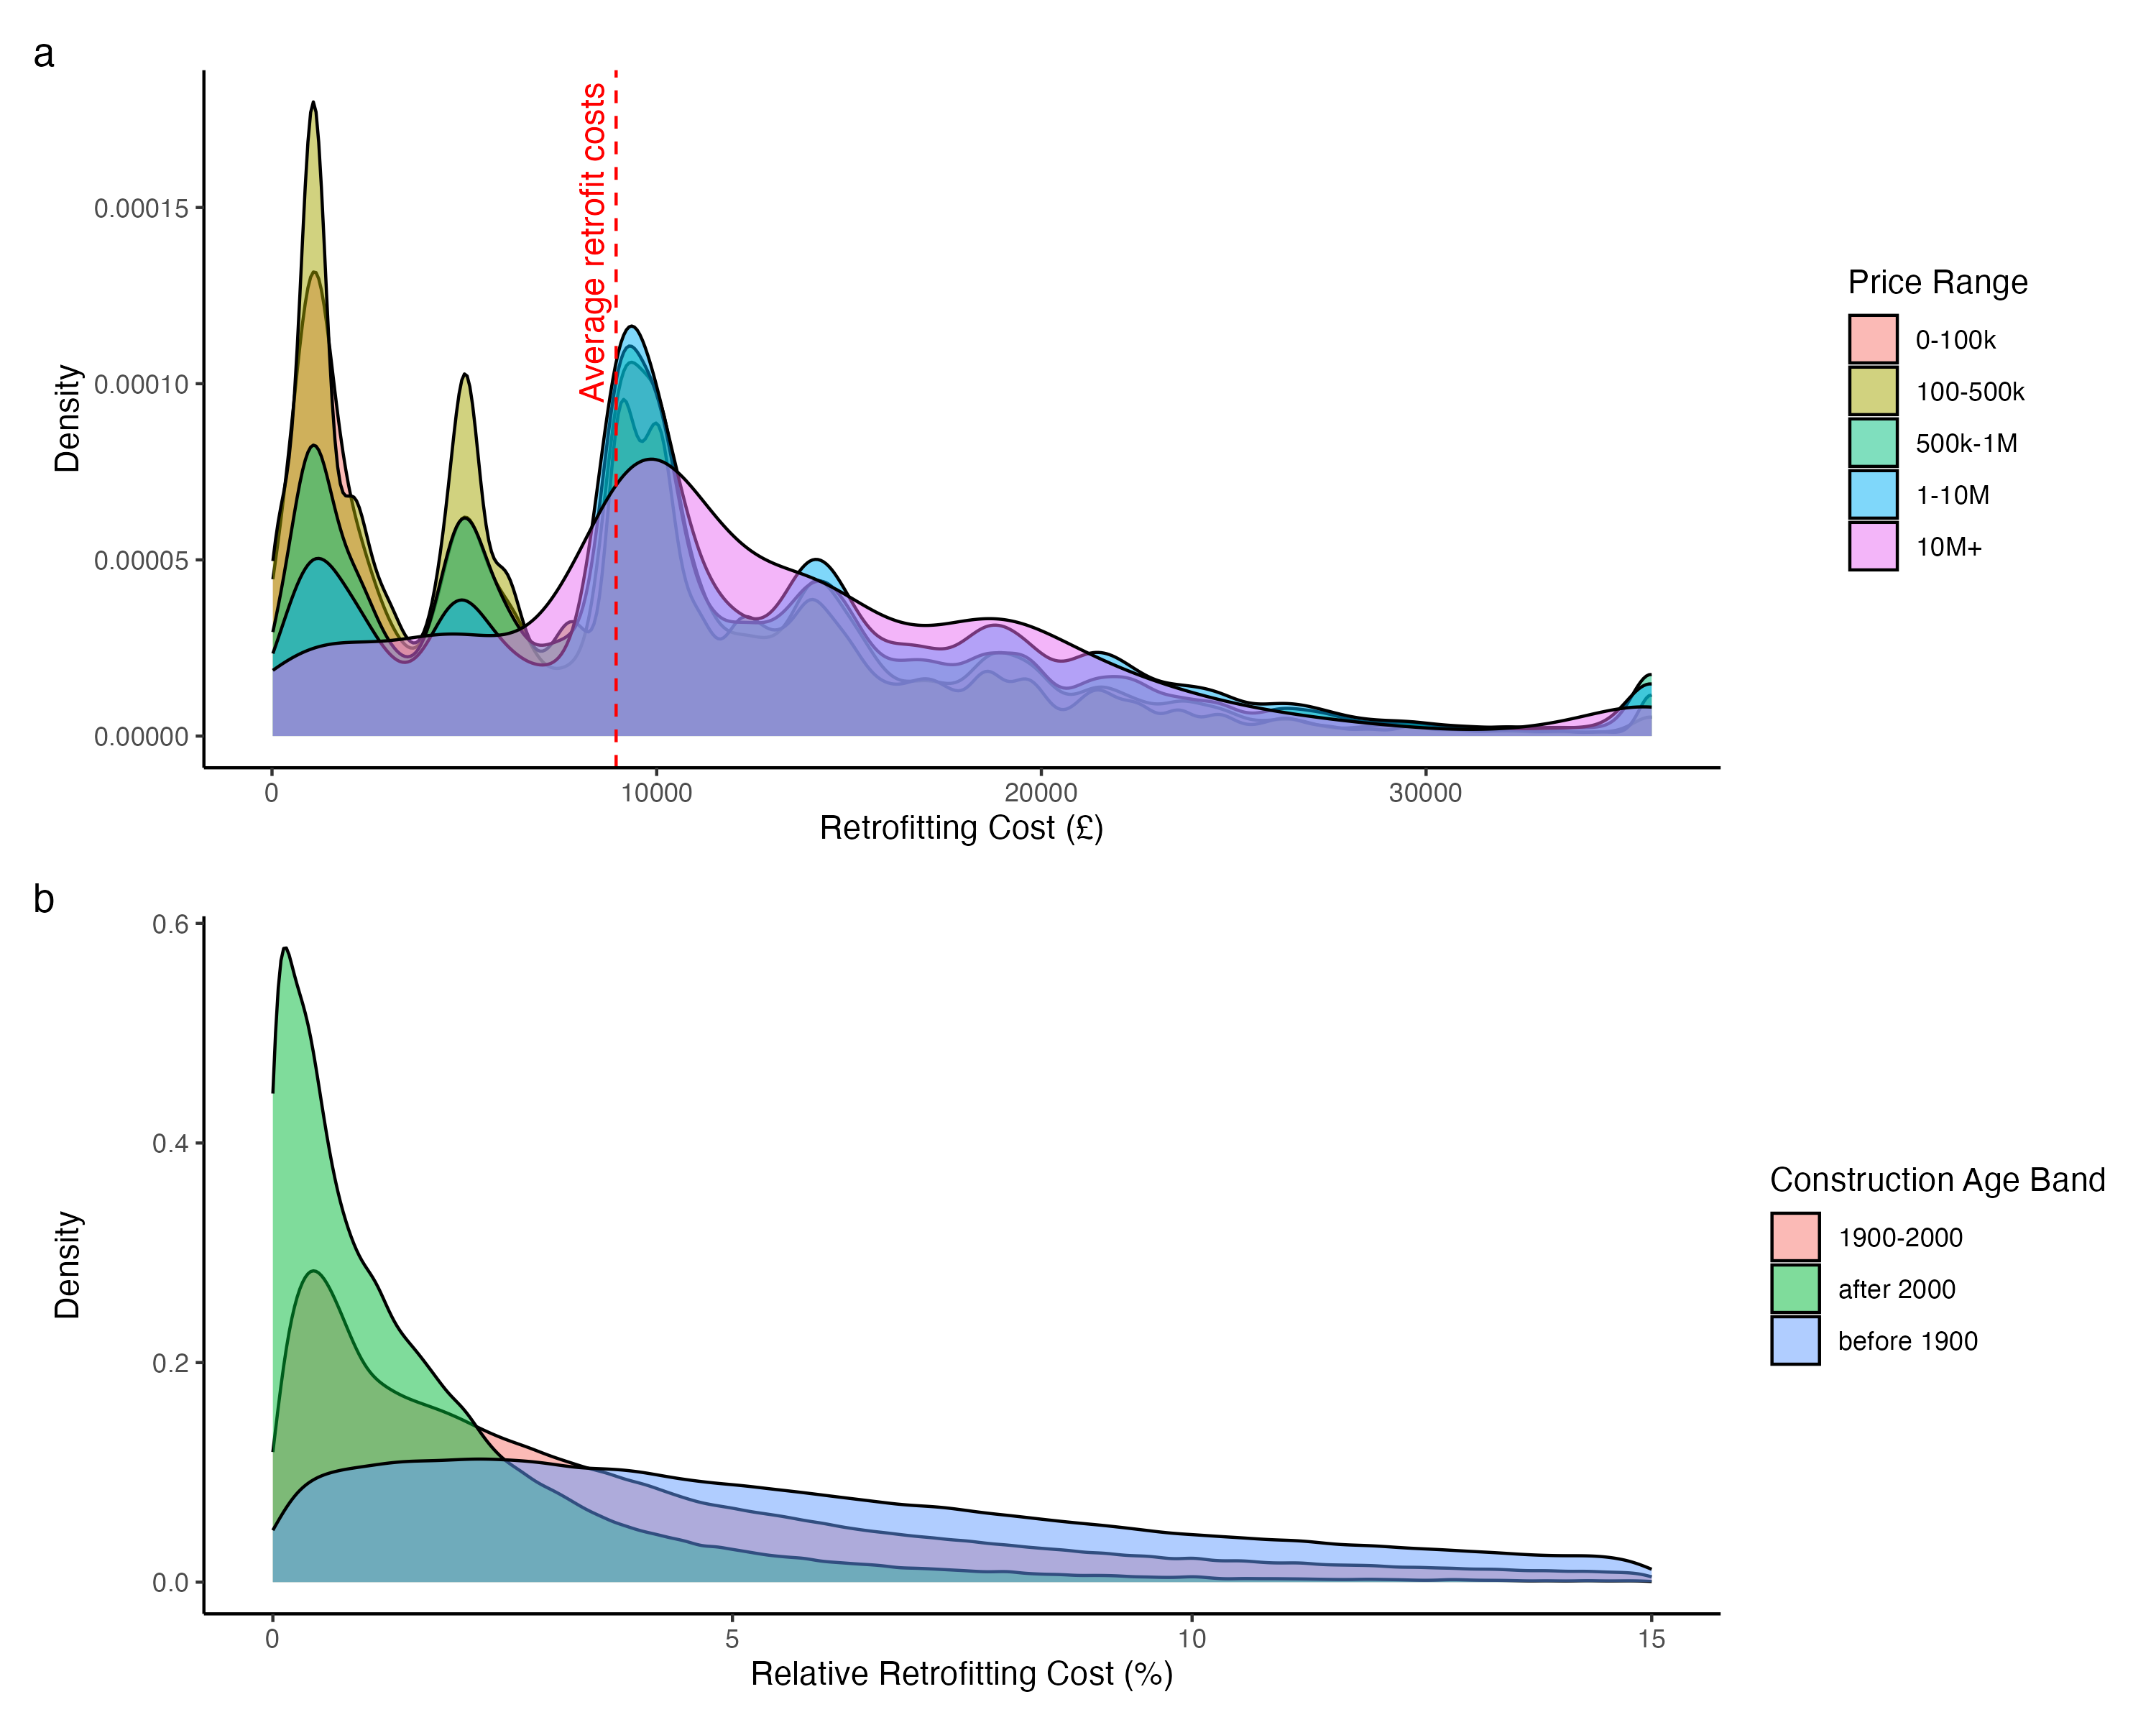
\includegraphics[width=1\linewidth]{src/figures/Combined_Density_Costs.png}
    \caption{Density plot of absolute (a.) and relative (b.) household retrofitting costs from following EPC recommendations (Strategy 1) to reach hypothetical MEES of EPC - C. Relative costs were determined as percent of property value as of latest transaction. The dashed line in subplot a. represents the average retrofitting cost per household according to this strategy (\textsterling 9,058 according to Table \ref{EPC_69_costs}). Top 1\% of properties with high retrofitting costs were excluded (winsorized at 99\%) to avoid outliers.}
    \label{fig:density_plot}
\end{figure}

\noindent While an estimate $15.6 $ million registered dwellings were considered 'able to improve their energy efficiency' according to their EPC \footnote{A dwelling considered 'able to improve' here refers to EPCs including improvement recommendations and a differing potential energy efficiency as outputted by the SAP software. } , $6$ million observations had above-standard energy efficiencies and $1$ million properties were unable to every reach a minimum C-Band energy rating (EPC Score of 69) as their 'potential energy efficiency' fell below such threshold. According to the 2015 Energy Efficiency Regulations, dwellings unable to meet MEES require to retrofit until reaching full energy efficiency potential or spending above the a maximum retrofitting budget set by the government. Retrofitting costs the all properties were then computed analogous methodologies and summarized in Table \ref{tab:table5_costsdescription}. 

% add unable to improve at all, and unable to spend at least 10k?
\begin{table}[h!]
\centering
\caption{Dwellings of various capacities to reach the potential MEES of EPC - C. }
\label{tab:table5_costsdescription}
\resizebox{\textwidth}{!}{ 
\begin{tabular}{lrrr}
\toprule
& \textbf{Already Achieved} & \textbf{Unable to Reach} & \textbf{Able to Reach EPC 69} \\
\midrule
\textbf{Number of Houses} & 6,368,752 & 1,060,889 & 8,171,825 \\
\textbf{Total Retrofit Costs} ($10^9$\textsterling) & - & 9.4 & 8.3 \\
\textbf{Reduced Emissions} ($MtCO_2{eq}/yr$) & - & -1.7 to - 2.0 & -12.8 to -20.6 \\
\addlinespace
\textbf{Average Retrofit Cost (\textsterling)$^*$} & - & 8,571 & 9,058 \\
Avg. \textit{pre-}retrofit EPC & 75 & 48 & 57 \\
Avg. \textit{post-}retrofit EPC & - & 61 & 69 \\
\addlinespace
\textbf{Average Property Price (\textsterling) } & 290,397 & 327,014 & 287,725 \\
\bottomrule
\end{tabular}
}
\begin{minipage}{\textwidth}
\scriptsize{\textit{\small{\textbf{NOTE: } For properties unable to reach EPC - C, retrofit costs were determined from maximum energy efficiency potential.}}}
\end{minipage}
\end{table}





\subsection{Green premium for energy efficiency} \label{Sec:green_premium}

\textbf{Green premium: 3 confounders (demand, supply and renovations/condition of the house at time of sale) we add interest rates, and listing data to take care of most important factors. 
need one more column with both interest rate and listing data.
listing were aggregated/counted active per area around a property 30 days (TBD) before transaction finalised as it takes an average of 3 months to complete.}

A  hedonic regression model was used to reveal the marginal effects of energy efficiency and other building characteristics at the time of sale on the transaction price. Hedonic price model was used to estimate willingness to pay using transaction price data \cite{harrison_hedonic_1978} using an adjusted OLS regressions of deflated prices ($P_{it}$ ) as a function of  the SAP score and attributes extracted from the EPC data ($X_{it}$):

\begin{align}
    \text{P}_{it} = \alpha_i + \beta_1 \cdot \text{EPC}_{it} + \sum_{j=2}^{8} \beta_j \cdot             \text{X}_{j,it} +  \gamma_t \cdot \text{time}_t + \epsilon_{it}
\label{Hedonic_m2}
\end{align}

Where \(\beta_{1:9}\) are the hedonic weights and $X_{it}$ are comprised of the total floor area ($X_2$), property type ($X_3$), number of habitable rooms ($X_4$), extension count ($X_5$),, building type ($X_6$), construction age band ($X_7$), and main fuel source ($X_8$) for each dwelling. These are included are control variables to limit omitted variables bias and improve the accuracy and  validity of the model \cite{wilms_omitted_2021}. $\epsilon_{it}$ refers to the standard error terms and, due to the large amount of transactions, is expected to follow a normal distribution. \\
Given that the total floor area is used in the SAP methodology to determine energy efficiency ratings \cite{bre_group_standard_nodate}, it is suspected to be correlated with energy efficiency, there is a concern of multicollinearity and endogeneity. Such concerns are also raised for construction age as part of the key determinants of energy demand, hence ultimately reflected in SAP ratings \cite{hamilton_energy_2013}. This correlation might inflate the estimates and obscure the true relationship between each variable and transaction price.  However the we assume the SAP methodology to take into account this step and provide the EPC ratings as 'fitted' values from building properties. Similarly, ages of dwellings have proven to be significantly correlated to energy efficiency as most houses built after 2012 are much more likely to be energy efficiency \cite{office_for_national_statistics_age_2022}. These potential sources of bias must be considered and taken into account when interpreting the regression results therein. \\

the hedonic price models were executed as OLS regressions using the \texttt{feos} plackage in R \cite{bergman_reframing_2020, berge_efficient_2018} on $10.4$ million transactions. The regressions results are displayed in table \ref{tab:hedonic_model}.  In line with expectations, the analysis reveals that energy efficiency is a statistically significant predictor of transaction price (p-value \textless 0.0001). In the simple hedonic model (Table \ref{tab:hedonic_model}), the coefficient associated with energy efficiency indicates a positive impact on transaction price, with an estimated hedonic premium of approximately £486.72 for every additional improvement in the Energy improvement score. Since the average improvement in energy efficiency across all properties is of 15, the estimates therein would result in an average net green premium of \textsterling $7,331.85$. This suggests that homes with higher energy efficiency ratings tend to command higher prices in the housing market, likely reflecting buyers' willingness to pay \cite{ghosh_homebuyers_2024}. \\

\begin{table}[ht]
\centering
\caption{Regression Results: Hedonic Price Models with Fixed Effects}
\resizebox{\textwidth}{!}{ 
\begin{tabular}{l c c c c}
\toprule
\toprule
& \textit{Simple Hedonic Model}  & \textit{Hedonic Model FE}  & \textit{With Interest Rates}  & \textit{With Listings} \\
\textit{Independent Variable}         & (1) & (2) & (3) & (4) \\
\midrule
Energy Efficiency & $500.88^{***}$ & $486.85^{***}$ & $483.26^{***}$ & $408.46^{***}$  \\
                  & $(5.54)$       & $(5.57)$       & $(5.56)$       & $(7.92)$        \\
\addlinespace
\midrule
Adj. R-Square     & $0.37$         & $0.37$         & $0.37$         & $0.45$          \\
N                 & $8,923,015$    & $8,923,015$    & $8,923,015$    & $4,001,425$     \\
\addlinespace
\midrule
Total Floor Area          & \textit{Yes}    & \textit{Yes}    & \textit{Yes}    & \textit{Yes}    \\
Property Type             & \textit{Yes}    & \textit{Yes}    & \textit{Yes}    & \textit{Yes}    \\
Number of Habitable Rooms & \textit{Yes}    & \textit{Yes}    & \textit{Yes}    & \textit{Yes}    \\
Extension Count           & \textit{Yes}    & \textit{Yes}    & \textit{Yes}    & \textit{Yes}    \\
Built Form                & \textit{Yes}    & \textit{Yes}    & \textit{Yes}    & \textit{Yes}    \\
Construction Age Band     & \textit{Yes}    & \textit{Yes}    & \textit{Yes}    & \textit{Yes}    \\
YEAR Time-Fixed Effects   & \textit{No}     & \textit{Yes}    & \textit{Yes}     & \textit{Yes}     \\
MONTH Time-Fixed Effects  & \textit{No}     & \textit{Yes}    & \textit{Yes}     & \textit{Yes}     \\
Monthly Interest Rates    & \textit{No}     & \textit{No}     & \textit{Yes}    & \textit{Yes}     \\
Active Listings           & \textit{No}     & \textit{No}     & \textit{No}     & \textit{Yes}    \\
\bottomrule
\bottomrule
\addlinespace
\end{tabular}
}
\begin{minipage}{\textwidth}
\scriptsize{\textit{\scriptsize{{\textbf{NOTES:} These estimates are the results of OLS regressions. The table reports the effect of energy efficiency score (out of 100) on property transaction prices (dependent variable). The coefficients represent the change (in \textsterling) in the dependent variable (price) per unit change in the independent variable (energy efficiency). The first column reports the results for the simple hedonic model without time fixed effect and the second column includes the time fixed effects. Regressions include household fixed effects, along with time controls in the second column. Columns (3) and (4) use monthly interest rates and average yearly sale listings by region as fixed effects, respectively. Robust standard errors in parentheses. Significance levels are indicated as $^{***}p<0.001$; $^{**}p<0.01$; $^{*}p<0.05$.}}}}
\end{minipage}
\label{tab:hedonic_model}
\end{table}


When accounting for time-varying controls through the use of other fixed effects, namely monthly interest rates and number of properties listed for sale in the same region, the estimate is reduced to approximately £207.80 (Table \ref{tab:hedonic_model}). The reduction in the coefficient suggests that the initial model may have overestimated the impact of energy efficiency by not accounting for unobserved, unit-specific characteristics that do not vary over time. When controlling for the supply of housing (measured by the number of listings), the adjusted $R^2$ value increased significantly compared to the other models. This improvement in the model's explanatory power underscores the importance of controlling for a broad range of factors that influence housing prices, beyond just energy efficiency. \\


\subsection{Elasticity of supply}
For this the sale price elasticity were parametrically estimated from the given active listings dataset \footnote{Zoopla Limited, © 2024 2. Zoopla Limited. Economic and Social Research Council. Zoopla Property Data, 2024 [data collection]. University of Glasgow - Urban Big Data Centre} from the equation below, similar to work done by \cite{malpezzi_long-run_2001}. Price elasticity refers to the effects of additional demand shocks on residential market prices and draws from the economic theory of "law of demand" \cite{fibich_dynamics_2005}.
\begin{align*}
    ln(P_i) = \beta \cdot ln(\text{active listings}_i) + \gamma_i \cdot t + rent_i : t_i
\end{align*}

According to the properties at risk and potential decision framework to sell or rent therein, over $500$ thousand properties risk entering the housing market for sale.\footnote{all properties with construction age before 1949 and in districts with high retrofitting cost and high fuel-poverty (nealry 2.6 million) and adjusted for the estimated 19\% of dwellings for rent} These refer to homes current renting that may be forced to sale faced with imposed MEES. This may have significant impacts on the UK housing market. According to the results (table \ref{table:coefficients}) elasticity is significant and is estimated that for every additional 1\% in active listings, property prices decrease by 2\%. Since about 8.1 million properties were currently listed in the market (from dataset), an additional 6.3\% properties might enter the market as a result of the MEES. Inducing a 11.3\% drop in property prices.
\begin{table}[ht]
\centering
\caption{Regression results showing the effects of base rate and other predictors on ln of growth\_price.}
\resizebox{0.3\textwidth}{!}{ 
\begin{tabular}{@{}l c@{}}
\toprule
\toprule
\textit{Independent Variables} & \textbf{House Price (\textsterling)} \\
\midrule
\addlinespace
\textbf{ln Active Sales}            & $-0.02^{**}$  \\
                                     & $(0.00)$      \\
\addlinespace                            
Interest Rates             & $0.02^{*}$    \\
                                     & $(0.01)$      \\
\addlinespace
Ajd. Interest Rates              & $-0.01^{*}$   \\
                                     & $(0.00)$      \\
\midrule
N.                    & $3,359,780$   \\
R$^2$        & $0.03$        \\
Adj R$^2$      & $0.01$        \\

\midrule
Property Type & \textit{yes}         \\
District   & \textit{yes}         \\
Year   & \textit{yes}       \\
Month       & \textit{yes}         \\

\bottomrule
\addlinespace    
\end{tabular}
}
\begin{minipage}{\textwidth}
\scriptsize{\textit{\scriptsize{{\textbf{NOTES:} These estimates are the results of OLS regressions. The table reports the effect of supply (number of active sales) on property transaction prices (dependent variable). Robust standard errors in parentheses. Significance levels are indicated as $^{***}p<0.001$; $^{**}p<0.01$; $^{*}p<0.05$.}}}}
\end{minipage}
\label{table:coefficients}
\end{table}


While the estimates above represent an immediate effect of the induced supply shock, which will inevitably decrease with time \cite{fibich_dynamics_2005}, it is highly significant. The increased supply of homes may have direct effects on the local housing prices but also have knock-on effects on neighbouring regions which buyers consider subsitutable \cite{fingleton_housing_2019} . This may have implications on the current housing crisis by increasing the supply of homes and potentially increase affordability across the UK.